\section{Keymaps alternatives}

\begin{frame}{Le Dvorak}
    \begin{itemize}
	\item Le dvorak, ou clavier americain simplifie (DSK).
	\item Concu par la methode Dvorak: en etudiant les langues cibles.
	\item Cree dans les annees 30 par August Dvorak et William Dealey.
	\newline
	\newline
	\pause
	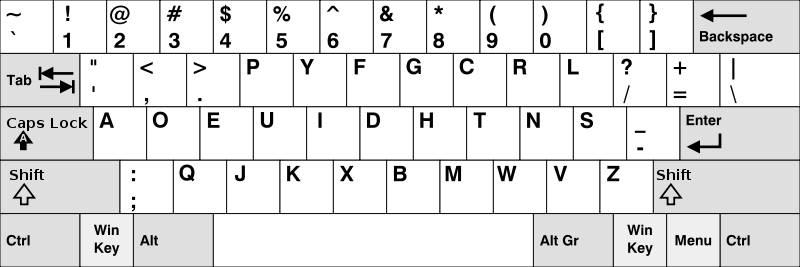
\includegraphics[height=90pt]{images/dvorak.png}
    \end{itemize}
\end{frame}

\begin{frame}{Le DSK}
    \begin{itemize}
	\item Clavier inadaptable pour d'autre langues.
	\item Quelques unes pour la france (Dvorak-fr, fr-Dvorak, Dvorak-international).
	\item Une seule tient la route: le bepo.
    \end{itemize}
    Quelques chiffres
    \begin{itemize}
	\item 70\% des lettres necessaires sont sur la ligne centrale.
	\item Procure confort et rapidite.
    \end{itemize}
\end{frame}
